\section{Experiment 4: Bars and Framed Rectangles}
\label{sec:barsframedrectangles}

Visual cues can help in converting graphical elements back to their real-world variables. Cleveland and McGill introduced the bars-and-framed-rectangles experiment to compare the perceptual judgment of length and position along non-aligned scales. Fig.~\ref{fig:figure12_mlae} shows both variations on the left. Without framing, it is difficult to judge which bar is larger (bottom). However, with a frame showing maximum length, this length judgment \change{can be} converted into a position judgment along non-aligned scales, which simplifies the perceptual problem.

Cleveland and McGill theorize that judging the framed whitespace could be considered a length rather than a position judgment. Given this, they relate the task to Weber's Law: the perceivable difference within a distribution is proportional to the initial size of the distribution~\cite{householder1940weber}. For this experiment, Weber's Law implies that humans can more easily measure the difference in the white scale since its initial size is small, whereas estimating the small change in lengths of the black bars is harder. The Just Noticeable Difference (JND) is higher when the initial stimulus is smaller in size. 

We set up the experiment as a two value regression task (Fig.~\ref{fig:figure12_mlae}). \change{Each bar length varies randomly by between 1 and 12 of 60 pixels, with each bar undergoing an individual vertical shift of up to 20 pixels. There are 132 different labels over 50,160 possible stimuli.}

%\subsection{Hypothesis}

\begin{hypolist}
	\item \textbf{H4.1} \textbf{Networks performance will improve with additional visual cues.} The original bar and framed rectangle setting shows how visual cues aid humans in mapping graphical elements to quantitative variables. This should be the same for feed-forward neural networks, as we give them more signal from which to learn.
\end{hypolist}

%\begin{figure}[t]
%	  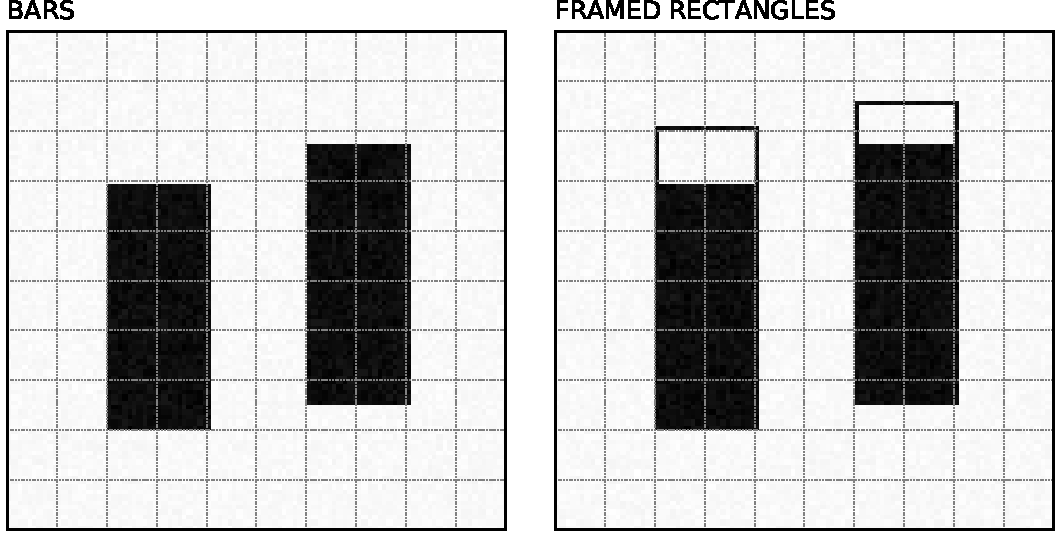
\includegraphics[width=\linewidth]{figure12_overview}
%  \caption{\textbf{Bars and Framed Rectangles Experiment.} Cleveland and McGill introduce the bars and framed rectangles experiment which measures the perceptual task of judging position along non-aligned scales. For humans, it is easier to decide which of two bars represent a larger height if a scale is introduced by adding framed rectangles (right). In this case, the right bar is heigher as visible with less free space when adding the frame. We evaluate whether such a visual aid also helps machines to perceive visually encoded quantities.}
%	\label{fig:bars_and_framed_rectangles_experiment}
%\end{figure}
%\begin{table}[h]
%\centering
%\caption{\textbf{Bars and Framed Rectangles Experiment.} Cleveland and McGill introduce the bars and framed rectangles experiment which measures the perceptual task of judging position along non-aligned scales. For humans, it is easier to decide which of two bars represent a larger height if a scale is introduced by adding framed rectangles. In this case, the right bar is heigher as visible with less free space when adding the frame. We evaluate whether such a visual aid also helps machines to perceive visually encoded quantities.}
%\resizebox{\linewidth}{!}{
%\begin{tabular}{lllr}
%	\toprule
%	\multicolumn{2}{l}{~} & ~ & Permutations\\
%
%	\midrule
%	\raisebox{-.85\height}{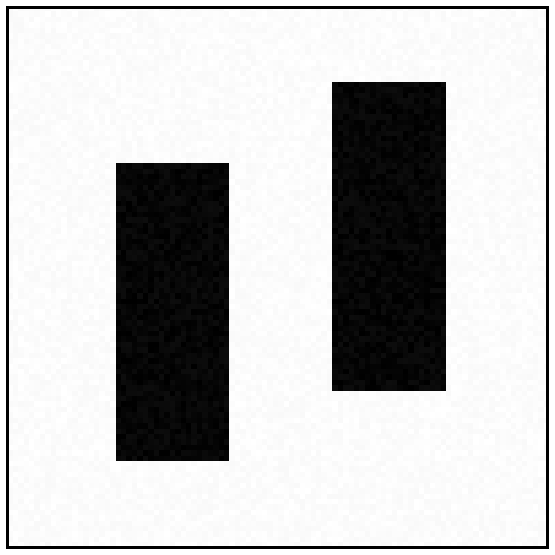
\includegraphics[width=.5in]{figure12_0.pdf}} & \makecell[tl]{\emph{Bars}\\~~~Perceptual Task: \emph{Length}\\~~~JND: $X\%$\\~ \\~~~~~~~~~~~~~~~~~~~~~~~~~~~~~~~~ \\} &~& \makecell[tr]{~\\ $57,600$}\\
%
%
%	\midrule
%	\raisebox{-.85\height}{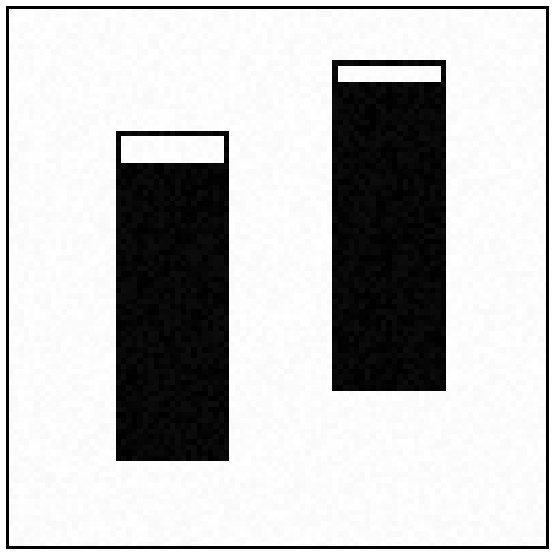
\includegraphics[width=.5in]{figure12_1.pdf}} & \makecell[tl]{\emph{Framed Rectangles}\\~~~Perceptual Task: \emph{Position}\\~~~JND: $X\%$\\~ \\~~~~~~~~~~~~~~~~~~~~~~~~~~~~~~ \\} &~& \makecell[tr]{~\\ $57,600$}\\
%
%
%	\bottomrule
%\end{tabular}
%}
%\label{tab:bars_and_framed_rectangles_parameters}
%\end{table}




%\begin{figure}[t]
%	  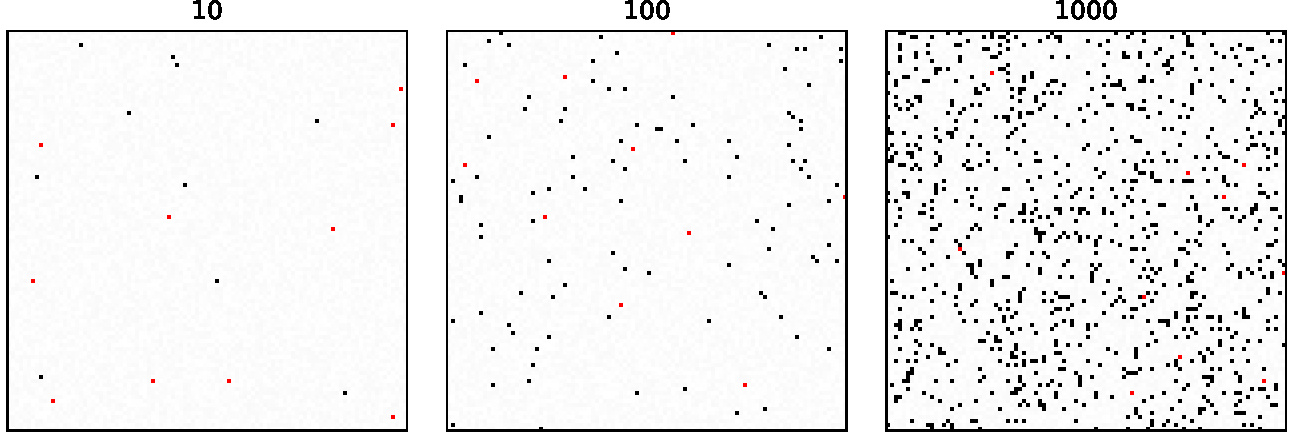
\includegraphics[width=\linewidth]{weber_overview}
%  \caption{\textbf{Weber-Fechner Law.} The Weber-Fechner law states that the perceivable differences within a distribution is proportional to the initial size of the distribution. The lower square contains 10 more dots than the upper one on both sides. However, the difference is easily perceivable on the left while the squares on the right almost look the same. We generate rasterized visualizations similar to this setup and evaluate our classifiers.}
%	\label{fig:webers_law}
%\end{figure}
%\begin{table}[h]
%\centering
%\caption{\textbf{Weber-Fechner Law.} The Weber-Fechner law states that the perceivable differences within a distribution is proportional to the initial size of the distribution. We create three different types of images initialized with 10, 100, and 1000 dots. We then mark randomly up to 10 dots in previously free pixels (here visualized in red). For humans, the difference is easily perceivable when the initial dot count is 10 but is hard when it is higher. We evaluate our classifiers on these rasterized visualizations.}
%\resizebox{\linewidth}{!}{
%\begin{tabular}{lllr}
%	\toprule
%	\multicolumn{2}{l}{~} & ~ & Permutations\\
%
%	\midrule
%	\raisebox{-.85\height}{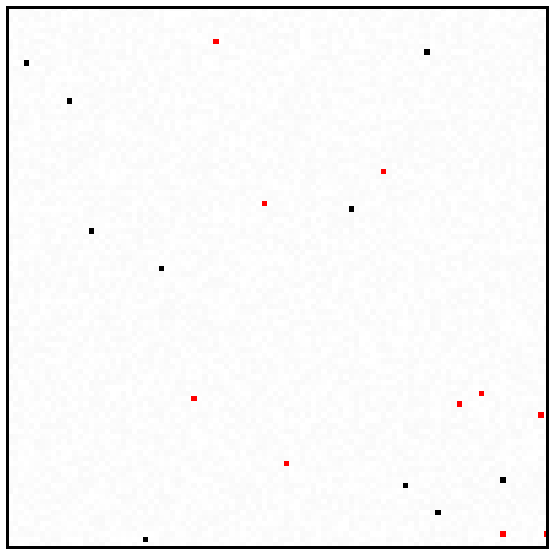
\includegraphics[width=.5in]{weber_0.pdf}} & \makecell[tl]{\emph{Base 10}\\~~~JND: $X\%$\\~ \\ ~~~~~~~~~~~~~~~~~~~~~~~~~~~~~~~~~~~~~~~~ \\} &~& \makecell[tr]{~\\ $10,000$}\\
%
%
%	\midrule
%	\raisebox{-.85\height}{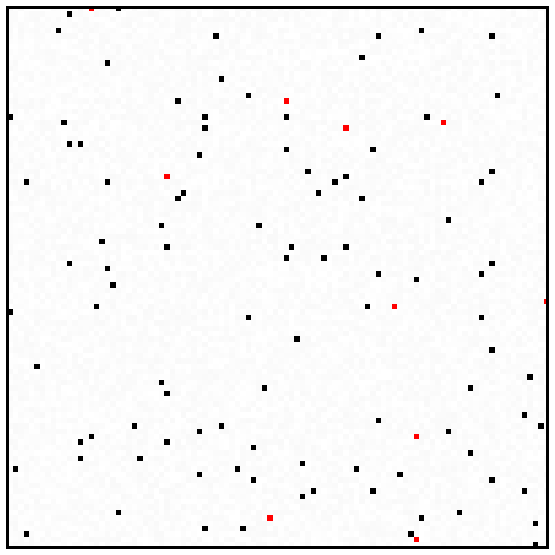
\includegraphics[width=.5in]{weber_1.pdf}} & \makecell[tl]{\emph{Base 100}\\~~~JND: $X\%$\\~ \\ ~~~~~~~~~~~~~~~~~~~~~~~~~~~~~~~~~~~~~~~~ \\} &~& \makecell[tr]{~\\ $10,000$}\\
%	
%	\midrule
%	\raisebox{-.85\height}{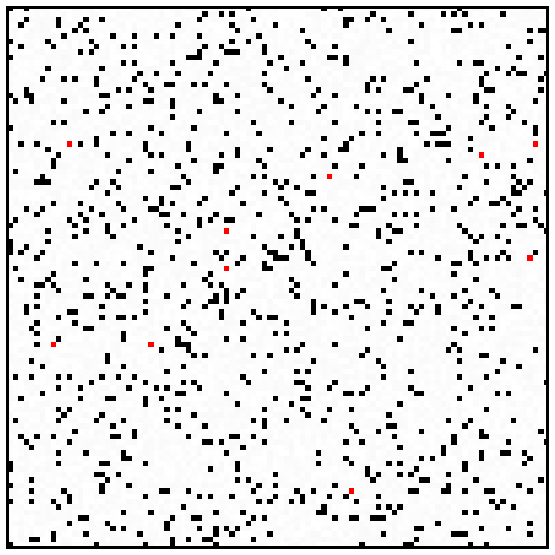
\includegraphics[width=.5in]{weber_2.pdf}} & \makecell[tl]{\emph{Base 1000}\\~~~JND: $X\%$\\~ \\ ~~~~~~~~~~~~~~~~~~~~~~~~~~~~~~~~~~~~~~~~ \\} &~& \makecell[tr]{~\\ $10,000$}\\
%
%	\bottomrule
%\end{tabular}
%}
%\label{tab:weber_law}
%\end{table}

\begin{figure}[tb]
  \centering
  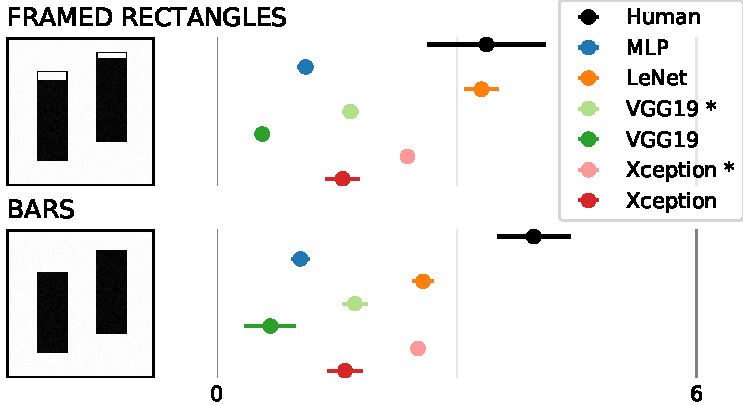
\includegraphics[width=0.9\linewidth]{figure12_mlae_better_all_NEW.pdf}
  \caption{\textbf{Computational results of the bars-and-framed-rectangles experiment.} \textit{Left:} Stimuli of two bars for length judgment (bottom) following Cleveland and McGill's setting. Perceiving which bar is longer is \change{significantly} easier for humans when a frame is added (top). \textit{Right:} For networks (trained from scratch, or * indicates ImageNet weights), there seems no significant difference between the encodings as reported by MLAE and \change{bootstrapped} 95\% confidence intervals.}
	\label{fig:figure12_mlae}
\end{figure}

\subsection{Results}

\change{Midmean random performance in this task is equal to $MLAE=4.8$.} We observe varying performance for our networks. Averaged across networks: the framed rectangle encoding $MLAE=1.982$ ($SD=0.89$) and for the bars encoding $1.867$ ($SD=0.709$). This difference was not significant, and so we \textbf{reject H4.1}. VGG19 again can regress the length in both cases, for the framed rectangle encoding $MLAE=0.595$ ($SD=0.225$) and for the bar encoding $MLAE=0.735$ ($SD=0.410$), though with higher variance without the added visual cues. The difference in relation to the visual cue is not significant. %\JT{Rejection of 4.1 calls into question the memorization of networks.}

\change{Further, our user study provides evidence that humans can more easily measure the frame rectangles. Participants were able to estimate the bar length with less error when frames are present $MLAE= 3.336 $ ($SD= 0.828 $) than without this visual aid $MLAE= 3.928 $ ($SD= 0.42 $). This difference is significant $F_{1,48}=9.765, p<0.01$.}

%\\~\\
%Unfortunately, both hypotheses were rejected for this experiment. However, it was great to see a partial validation of our ranking of elementary perceptual tasks (Table~\ref{tab:ranking}).

